\documentclass[tikz, dvipdfmx]{standalone}
\usepackage{tikz}

\usetikzlibrary{intersections,calc,arrows.meta}
\begin{document}
  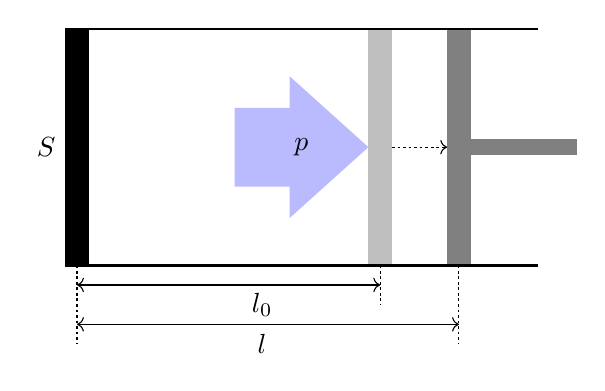
\begin{tikzpicture}
    %\begin{scope}[scale = 0.5]
    \fill[gray] (1.85,1.5) rectangle (2.15,-1.5);
    \fill[gray] (2.1,0.1) rectangle (3.5,-0.1);
    \fill[gray, opacity=0.5, shift={(-1,0)}] (1.85,1.5) rectangle (2.15,-1.5);
    \draw[->, dash pattern=on 1pt off 1pt] (1.15,0) -- (1.85,0);
    \draw[line width=1pt] (3,1.5) -- (-3,1.5);
    \fill (-3,1.5) rectangle (-2.7,-1.5);
    \draw[line width=1pt](-3,-1.5) -- (3,-1.5);
    \fill[blue!30!white, opacity=0.9, shift={(-2.05,0)}] (1.2,0.5) -- (1.2,-0.5) --(1.9,-0.5) -- (1.9,-0.9) -- (2.9,0) --(1.9,0.9) -- (1.9,0.5) -- cycle;
    \draw[dash pattern=on 1pt off 1pt] (1,-1.5) -- (1,-2);
    \draw[dash pattern=on 1pt off 1pt] (2,-1.5) -- (2,-2.5);
    \draw[dash pattern=on 1pt off 1pt] (-2.85,-1.5) -- (-2.85,-2.5);
    \draw[<->] (-2.85,-1.75) -- (1,-1.75);
    \draw[<->] (-2.85,-2.25) -- (2,-2.25);
    \draw (-0.5,-2) node{$l_0$};
    \draw (-0.5,-2.5) node{$l$};
    \draw (-3,0) node[left]{$S$};
    \draw (0,0) node{$p$};
  \end{tikzpicture}
\end{document}
